\documentclass[tikz,border=10pt]{standalone}
\usetikzlibrary{intersections}
\begin{document}
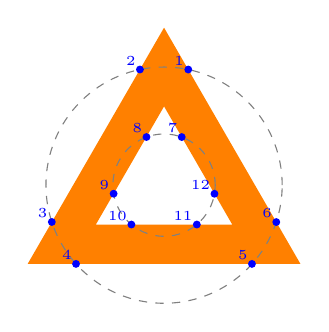
\begin{tikzpicture}
  \fill[name path=triangle, orange]
    (90:2) -- (210:2) -- (330:2) -- cycle
    (90:1) -- (330:1) -- (210:1) -- cycle;
  \draw[name path=circle, dashed, gray]
    circle(1.5) circle(0.65);
  \fill[blue,
    name intersections = {of = triangle and circle,
    total=\max, name=c, sort by = circle}]
    \foreach \i in {1,...,\max} {
      (c-\i) circle(0.5mm)
      node[above left=0.5mm,font=\tiny, inner sep=0]{\i}};
\end{tikzpicture}
\end{document}
